\documentclass[11pt]{beamer}

\graphicspath{{assets/}{./}}

\usepackage{booktabs}
\usepackage{multicol}
\usepackage{tikz}
\usetikzlibrary{positioning}
\usepackage[utf8]{inputenc}
\usepackage[T1]{fontenc}
\usepackage{amsmath}
\usepackage{graphicx}
\usepackage[english]{babel}

\usetheme{Madrid}

\usepackage{csquotes}
% --- BIBLIOGRAPHY SETTINGS ---
\usepackage[backend=biber,style=numeric,sorting=none]{biblatex}
\addbibresource{references.bib} 

% Script to make bibliography font smaller for Beamer
\setbeamerfont{bibliography item}{size=\tiny}
\setbeamerfont{bibliography entry author}{size=\tiny}
\setbeamerfont{bibliography entry title}{size=\tiny}
\setbeamerfont{bibliography entry location}{size=\tiny}
\setbeamerfont{bibliography entry note}{size=\tiny}

% -------- FOOTER PERSONALIZADO --------
\newcommand{\eventname}{MEA 2026}

\setbeamertemplate{footline}{
  \leavevmode%
  \hbox{%
    \begin{beamercolorbox}[wd=.33\paperwidth,ht=2.7ex,dp=1.2ex,leftskip=0.8em]{author in head/foot}%
      \usebeamerfont{author in head/foot}\insertshortauthor
    \end{beamercolorbox}%
    
    \begin{beamercolorbox}[wd=.34\paperwidth,ht=2.7ex,dp=1.2ex,center]{title in head/foot}%
      \usebeamerfont{title in head/foot}\eventname
    \end{beamercolorbox}%
    
    \begin{beamercolorbox}[wd=.33\paperwidth,ht=2.7ex,dp=1.2ex]{date in head/foot}%
      \hfill
      \usebeamerfont{date in head/foot}
      \ifx\insertsection\empty
        \eventname
      \else
        \insertsection
      \fi
      \hspace{0.5em} | \hspace{0.5em}
      \insertframenumber/\inserttotalframenumber
      \hspace{0.8em}
    \end{beamercolorbox}%
  }%
  \vskip0pt%
}

\usefonttheme{default}
\usepackage{palatino}
\usepackage[default]{opensans}
\useinnertheme{circles}

% --- UPRM Green ---
\usepackage{xcolor}
\definecolor{uprmgreen}{RGB}{0,102,51}
\setbeamercolor{structure}{fg=uprmgreen}

% Avoid hyperref warnings
\pdfstringdefDisableCommands{%
  \def\\{}%
  \def\and{, }%
}

%------------------------------------------------
% TITLE INFORMATION
%------------------------------------------------

\title{The Association Between the Kaitz Index and Employment in Puerto Rico}
\subtitle{A Spatial Durbin Model Approach}

\author[Ouslan]{\small{
  Alejandro M. Ouslan \& Dr. Julio C. Hernández}\\
}

\institute[UPRM]{University of Puerto Rico, Mayagüez}
\titlegraphic{
\includegraphics[width=2cm]{logo_UPRM.pdf}}

\date[\today]{\small{Annual Meetings of the Midwest Economics Association}\\
\vspace{2mm}
\footnotesize{\today}}

%------------------------------------------------
% CUSTOM TITLE PAGE
%------------------------------------------------

\setbeamertemplate{title page}{
  \vbox{}
  \vfill
  \begin{center}

    \begin{beamercolorbox}[sep=12pt,center,rounded=true,shadow=true]{title}
      {\usebeamerfont{title}\inserttitle\par}
    \end{beamercolorbox}

    \vspace{0.4cm}

    {\usebeamerfont{author}\insertauthor\par}

    \vspace{0.3cm}

    \inserttitlegraphic

    \vspace{0.3cm}

    {\usebeamerfont{date}\insertdate\par}

  \end{center}
  \vfill
}

%------------------------------------------------
\begin{document}

{
\setbeamertemplate{footline}{}
\setbeamertemplate{headline}{}
\begin{frame}
	\titlepage
\end{frame}
}

%------------------------------------------------
% TABLE OF CONTENTS
%------------------------------------------------

\section*{Presentation Overview}
\begin{frame}{Presentation Overview}

	\begin{columns}[T,onlytextwidth]
		\column{0.5\textwidth}
		\tableofcontents[sections={1-3}]

		\column{0.5\textwidth}
		\tableofcontents[sections={4-6}]
	\end{columns}

\end{frame}

%------------------------------------------------
\section{Introduction}
%------------------------------------------------

\begin{frame}{Research Context}
	\begin{itemize}
		\item \textbf{Objective:} Examine the relationship between the Kaitz Index and employment levels in Puerto Rico.
		\item \textbf{Data:} Panel data at the postal code (ZIP) level from Q1 2012 to Q4 2023.
		\item \textbf{Key Gap:} Exploring the \textbf{spatial dynamics}—how wage conditions in one region affect neighboring areas.
		\item \textbf{Methodology:} Spatial Durbin Model (SDM) with Fixed Effects.
	\end{itemize}
\end{frame}

%------------------------------------------------
\section{Literature Review}
%------------------------------------------------

\begin{frame}{Literature Summary}
	\begin{itemize}
		\item \textbf{Negative Relationship:} Freeman (1992) \cite{castillo1992minimum} found 8\%--10\% employment reduction; Neumark (2000) \cite{neumark2000minimum} linked high minimum wages to high unemployment.
		\item \textbf{Mixed Results:} Card \& Krueger (1994) \cite{card1994comment} found no significant effect; Caraballo-Cueto (2016) \cite{caraballo2016there} observed slight positive short-run effects.
		\item \textbf{Puerto Rico Specific:} Federal Reserve (2012) \cite{torres2012competitividad} suggested subminimum wages; Hernández (2017) found reductions post-increase.
	\end{itemize}
\end{frame}

%------------------------------------------------
\section{Methodology}
%------------------------------------------------

\begin{frame}{Defining the Kaitz Index}
	The Kaitz Index ($K$) represents the ratio of the minimum wage to the average wage:

	\[
		K_{it} = \frac{m_t}{\bar{w}_{it}}
	\]

	\begin{block}{Variables}
		\begin{itemize}
			\item $m_t$: Minimum wage at time $t$.
			\item $\bar{w}_{it}$: Average wage in zip code $i$ at time $t$.
		\end{itemize}
	\end{block}
	\textit{Source: FRED and QCEW (Department of Labor).}
\end{frame}

\begin{frame}{Spatial Durbin Model (SDM)}
	To account for spatial dependence, we use \cite{lee2016identification}:
	\[
		Y_{it} = \alpha + \beta_1 X_{it} + \rho W Y_{it} + \gamma W X_{it} + \epsilon_{it}
	\]
	\begin{itemize}
		\item $Y_{it}$: Employment in zip code $i$.
		\item $W$: Spatial weights matrix (Adjacency).
		\item $\rho$: Spatial autoregressive parameter.
		\item $\gamma W X_{it}$: Spatial lags of independent variables (Indirect effects).
	\end{itemize}
\end{frame}

\begin{frame}{Spatial Weighting Strategies ($W$)}
	Four distinct weights are implemented for robustness:
	\begin{enumerate}
		\item \textbf{$W_{queen}$}: Contiguous borders.
		\item \textbf{$W_{knn6}$}: 6 nearest neighboring regions.
		\item \textbf{$W_{distance}$}: 30-mile radius.
		\item \textbf{$W_{tensor}$}: Semi-parametric diagnostic using centroids to check for non-uniform spatial correlation.
	\end{enumerate}
\end{frame}

%------------------------------------------------
\section{Results}
%------------------------------------------------

\section{Results: Queen Adjacency}
\begin{frame}{Queen Weights: Parameter Estimates}
	\begin{table}
		\centering
		\tiny
		\begin{tabular}{lccc|c}
			\toprule
			\textbf{Variable} & \textbf{Mean} & \textbf{3\% CI (L)} & \textbf{3\% CI (U)} & \textbf{R-Hat} \\
			\midrule
			Kaitz Index       & -9.594        & -12.806             & -6.093              & 1.00           \\
			Sigma             & 8.164         & 8.013               & 8.300               & 1.00           \\
			Intercept         & 13.808        & 3.715               & 23.321              & 1.01           \\
			Commute by Car    & -0.001        & -0.001              & -0.000              & 1.01           \\
			WQ Employment     & -0.040        & -0.106              & 0.036               & 1.00           \\
			WQ K Index        & -1.139        & -8.625              & 7.089               & 1.00           \\
			\bottomrule
		\end{tabular}
	\end{table}
\end{frame}

\begin{frame}{Queen Weights: Posterior Distribution}
	\begin{figure}
		\centering
		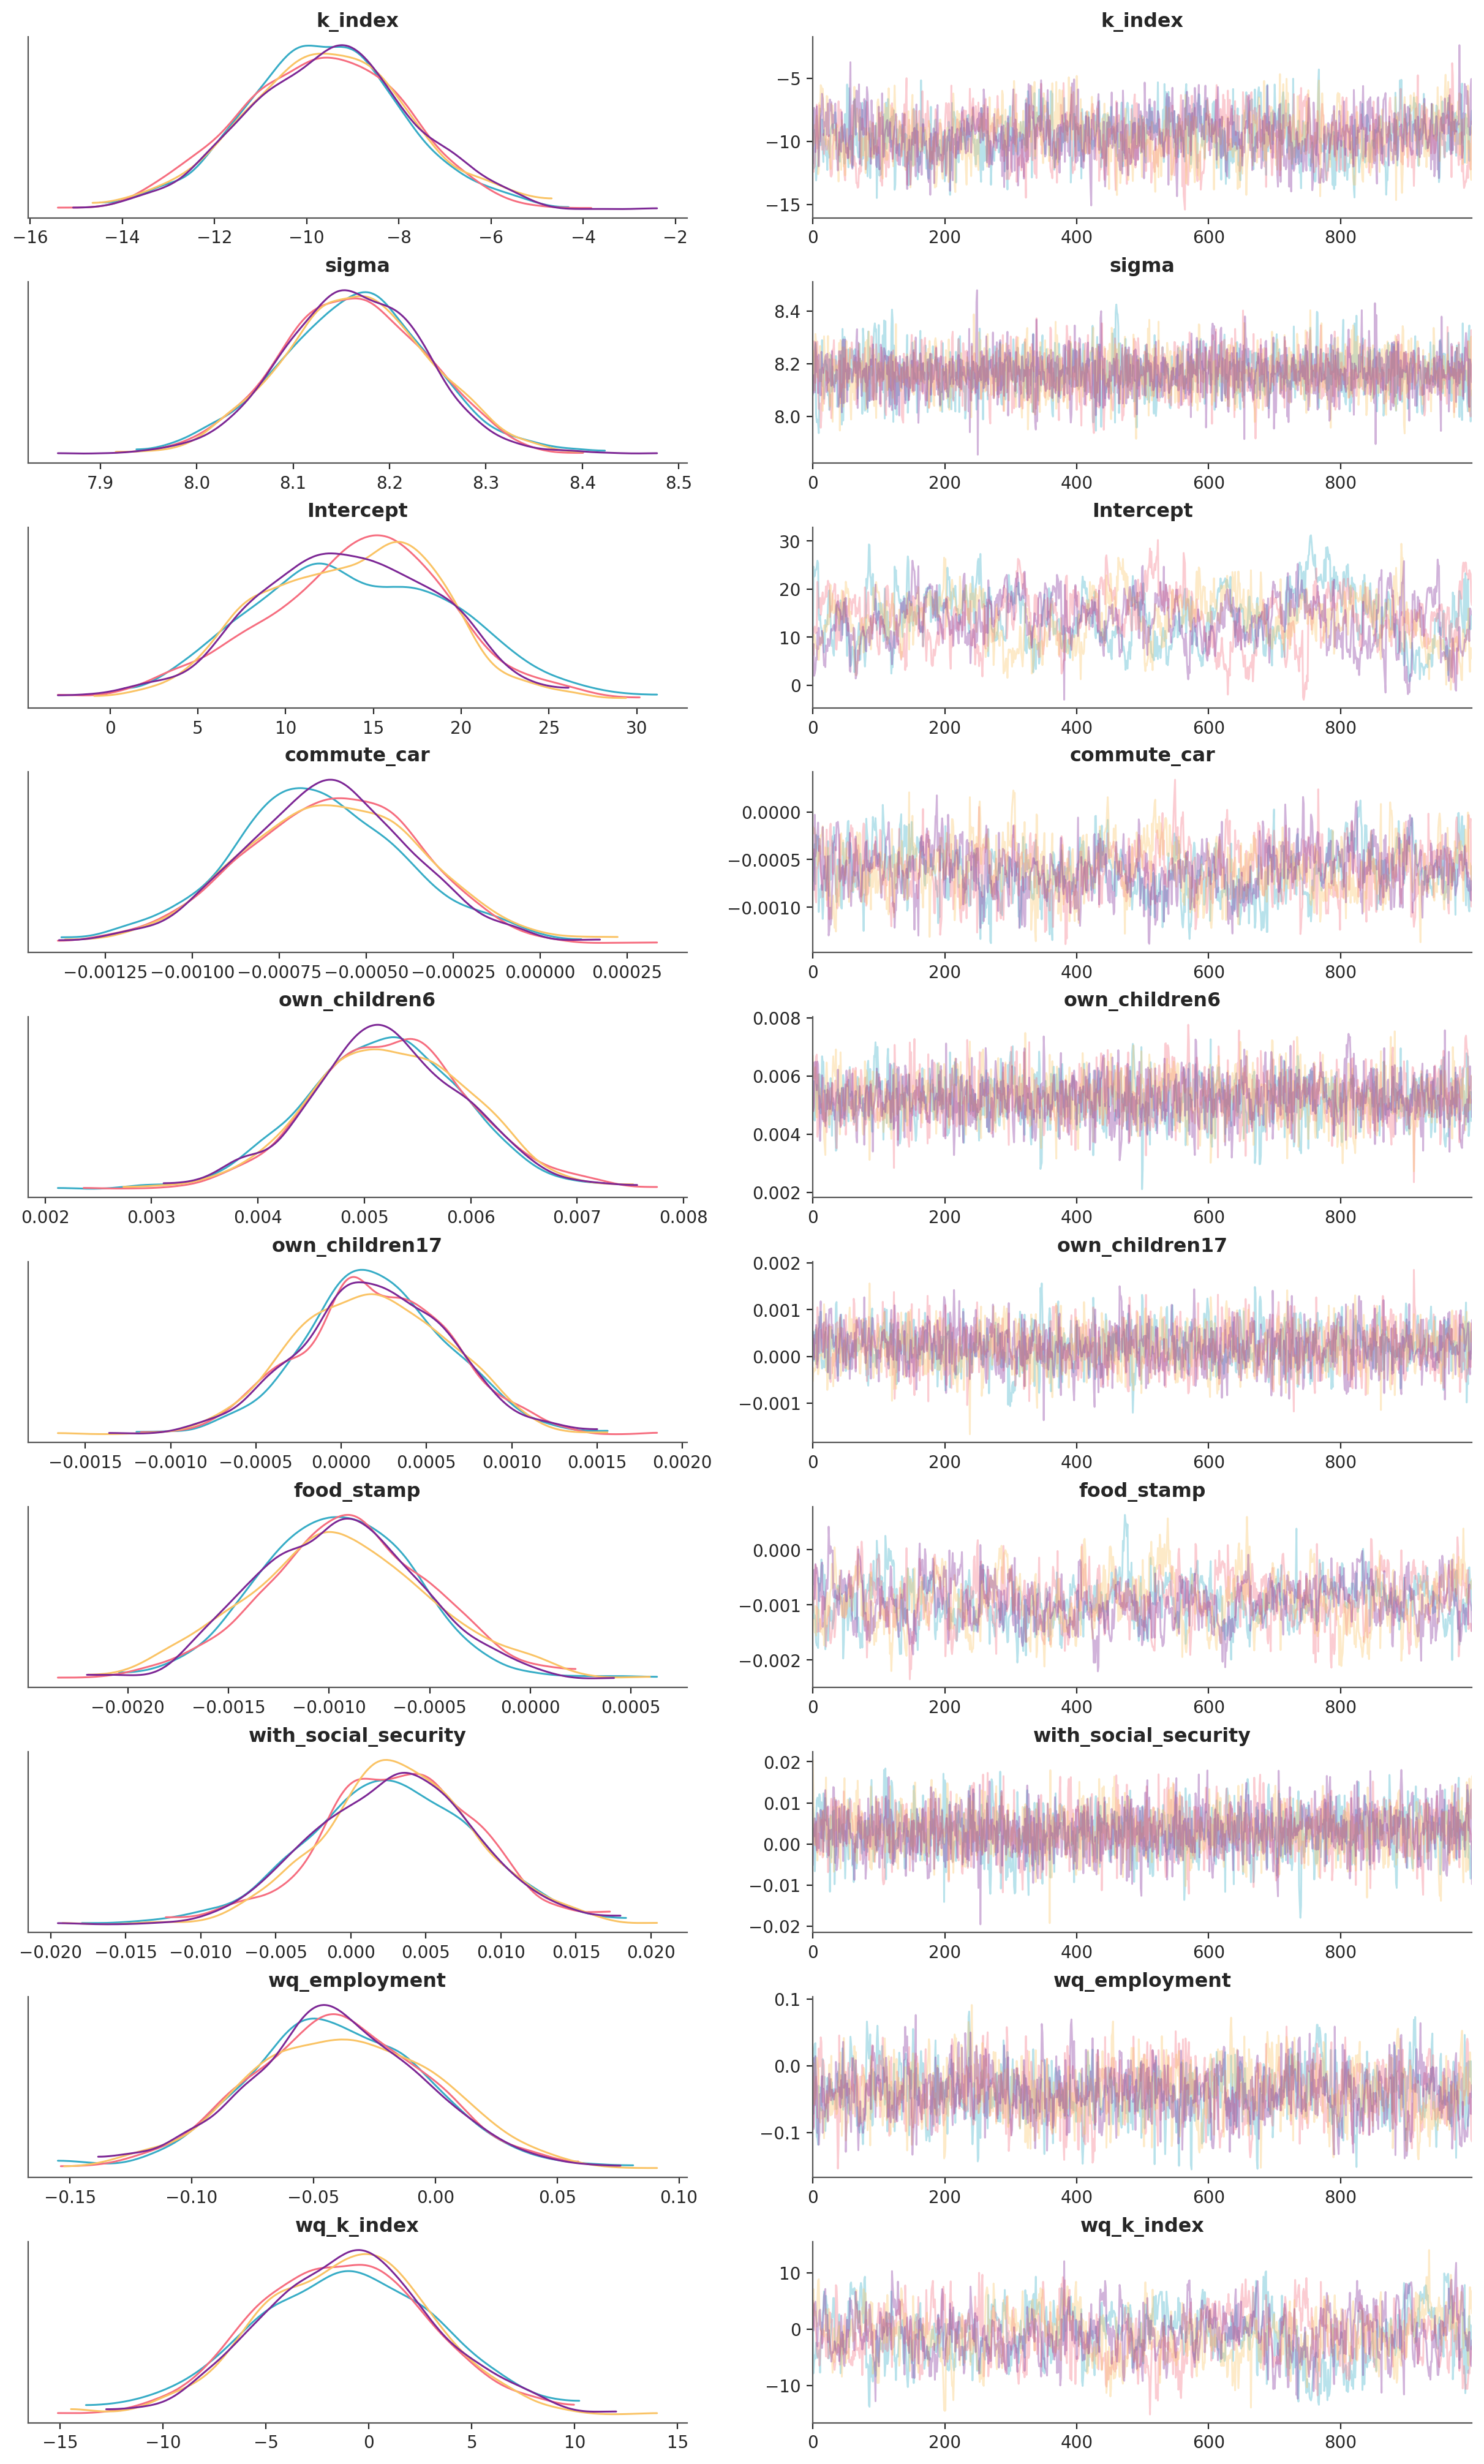
\includegraphics[width=0.4\textwidth]{assets/queen_posterior.png}
		\caption{Regression Summary (Queen)}
	\end{figure}
\end{frame}

\section{Results: K-Nearest Neighbors (KNN6)}
\begin{frame}{KNN6 Weights: Parameter Estimates}
	\begin{table}
		\centering
		\tiny
		\begin{tabular}{lccc|c}
			\toprule
			\textbf{Variable} & \textbf{Mean} & \textbf{3\% CI (L)} & \textbf{3\% CI (U)} & \textbf{R-Hat} \\
			\midrule
			Kaitz Index       & -9.687        & -12.917             & -6.293              & 1.02           \\
			Sigma             & 8.163         & 8.015               & 8.307               & 1.00           \\
			Intercept         & 14.758        & 4.748               & 25.399              & 1.11           \\
			WK6 Employment    & 0.044         & -0.031              & 0.113               & 1.02           \\
			WK6 K Index       & -2.916        & -11.209             & 5.525               & 1.08           \\
			\bottomrule
		\end{tabular}
	\end{table}
\end{frame}

\begin{frame}{KNN6 Weights: Posterior Distribution}
	\begin{figure}
		\centering
		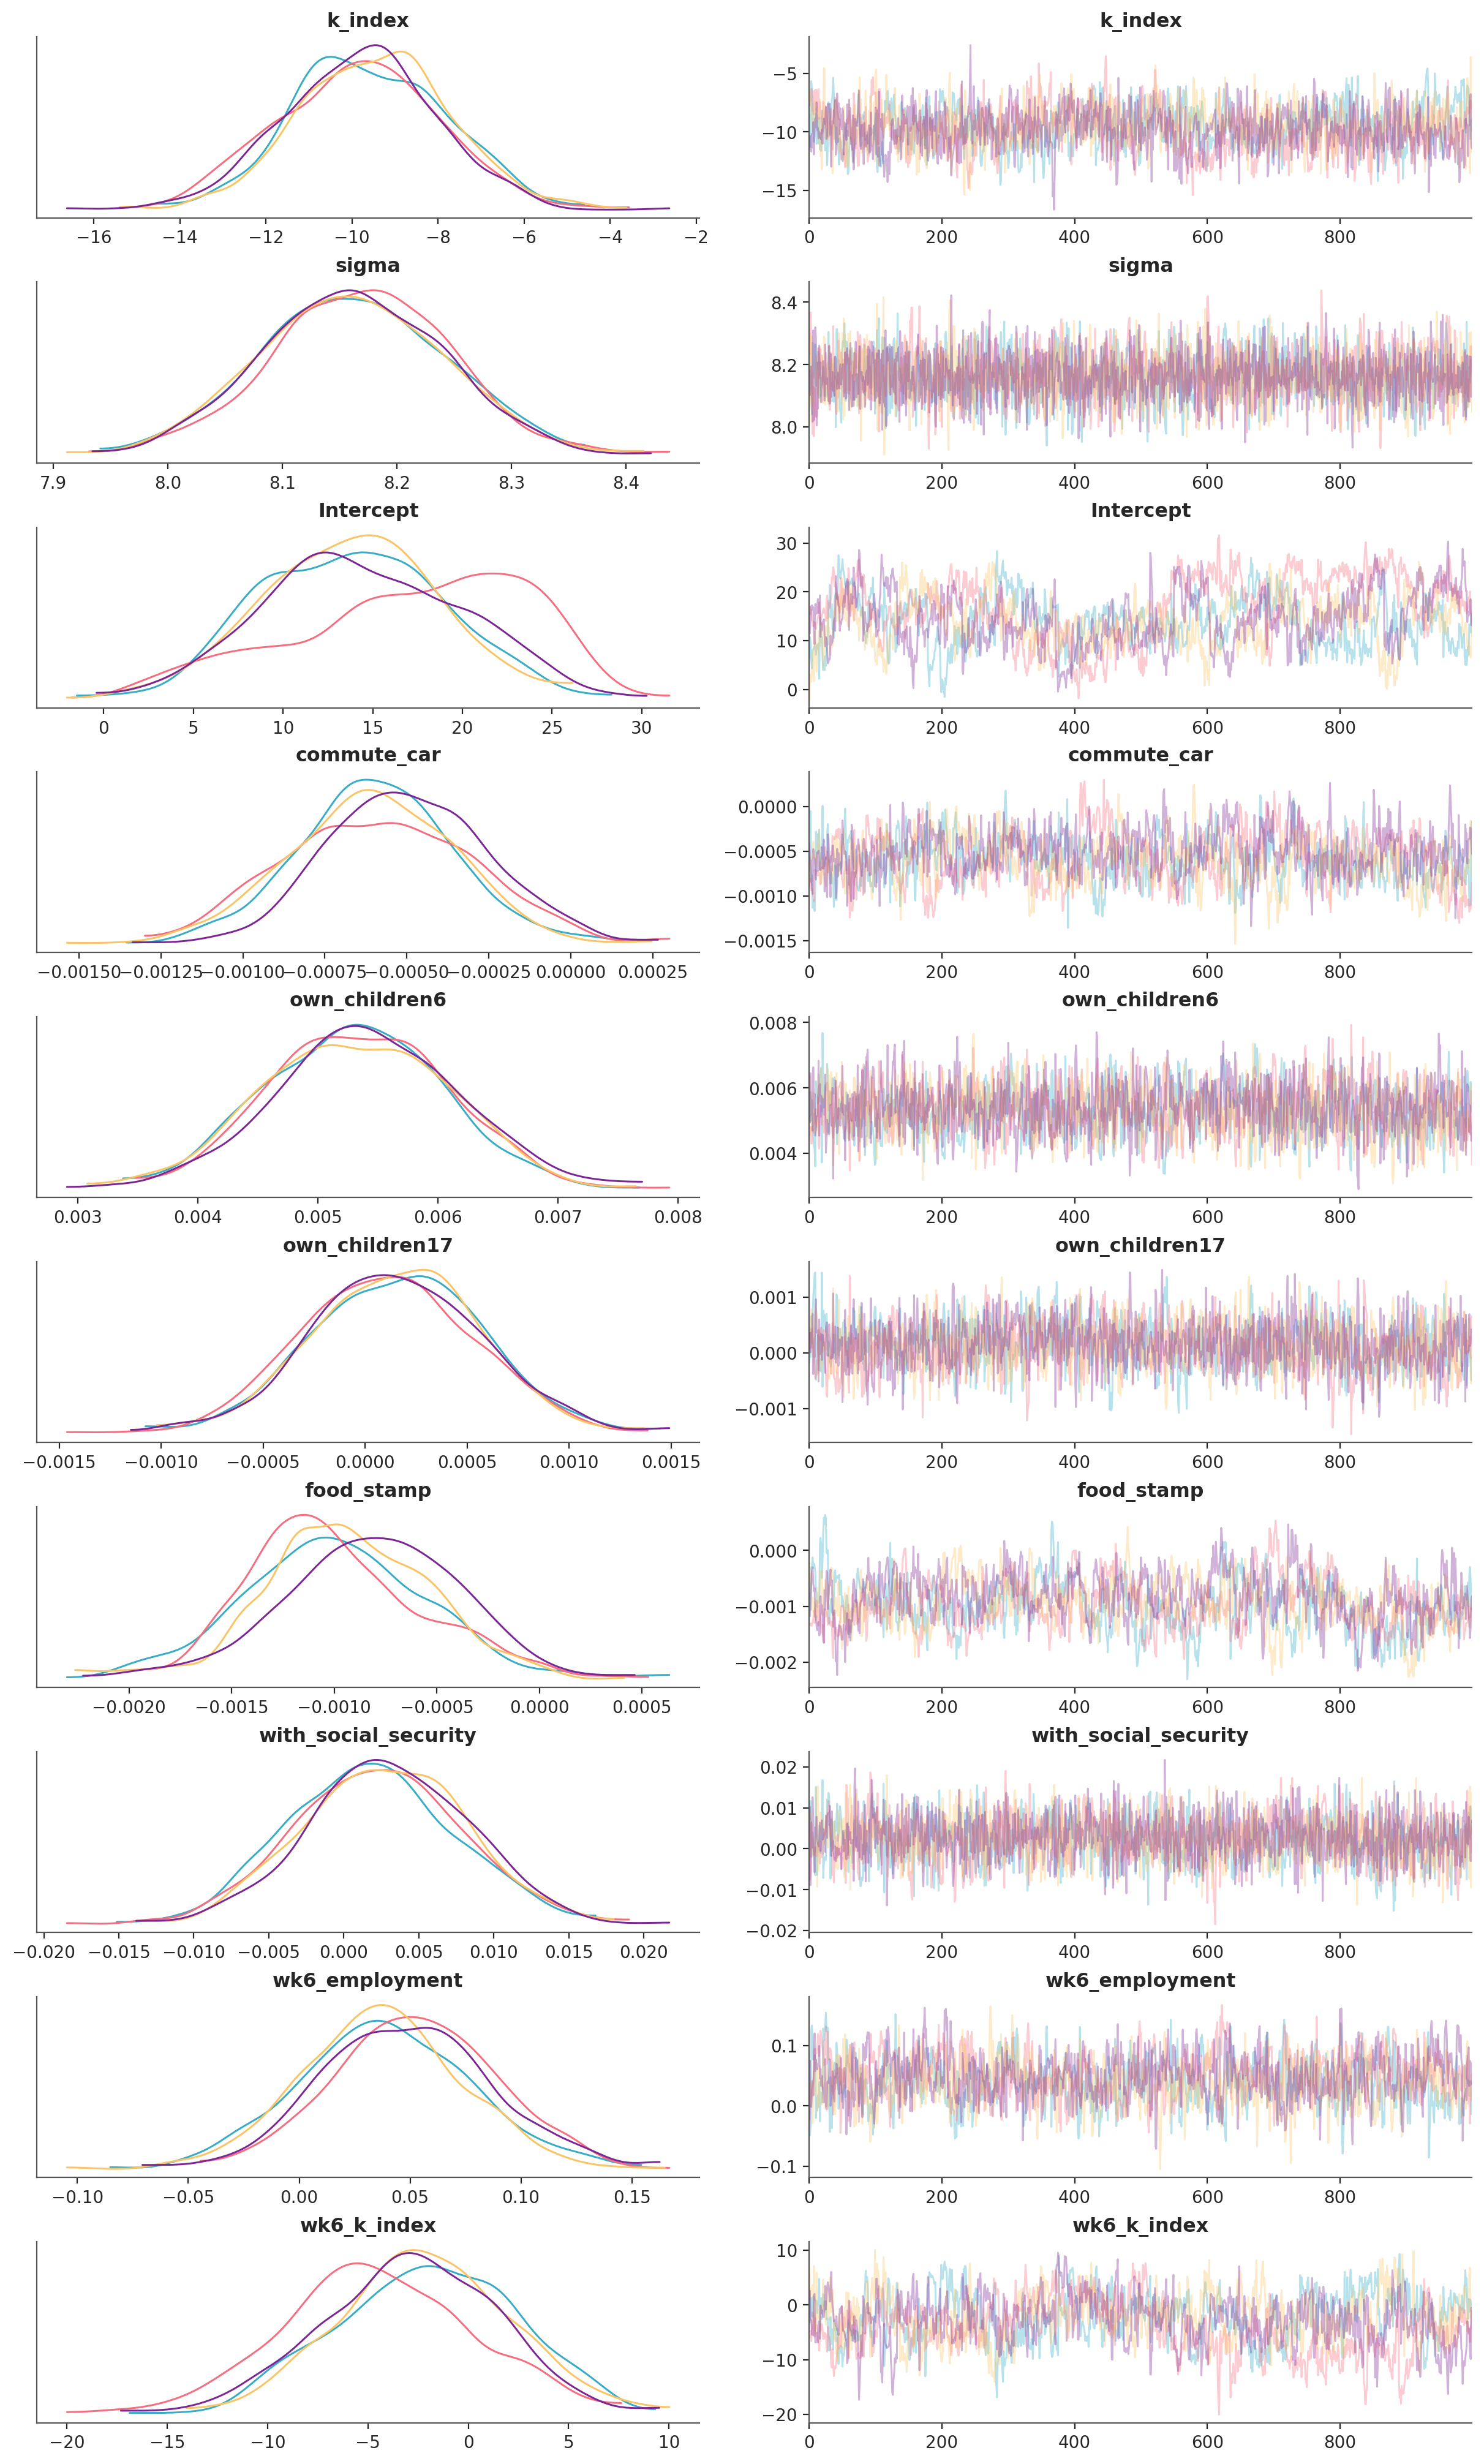
\includegraphics[width=0.4\textwidth]{assets/knn6_posterior.png}
		\caption{Regression Summary (KNN6)}
	\end{figure}
\end{frame}

\section{Results: Distance (30 Miles)}
\begin{frame}{Distance Weights: Parameter Estimates}
	\begin{table}
		\centering
		\tiny
		\begin{tabular}{lccc|c}
			\toprule
			\textbf{Variable} & \textbf{Mean} & \textbf{3\% CI (L)} & \textbf{3\% CI (U)} & \textbf{R-Hat} \\
			\midrule
			Kaitz Index       & -9.650        & -13.154             & -6.244              & 1.03           \\
			Sigma             & 8.160         & 8.009               & 8.307               & 1.00           \\
			Intercept         & 17.368        & -5.015              & 45.195              & 1.03           \\
			WD30 Employment   & -0.301        & -0.519              & -0.090              & 1.01           \\
			WD30 K Index      & -0.084        & -28.740             & 23.926              & 1.04           \\
			\bottomrule
		\end{tabular}
	\end{table}
\end{frame}

\begin{frame}{Distance Weights: Posterior Distribution}
	\begin{figure}
		\centering
		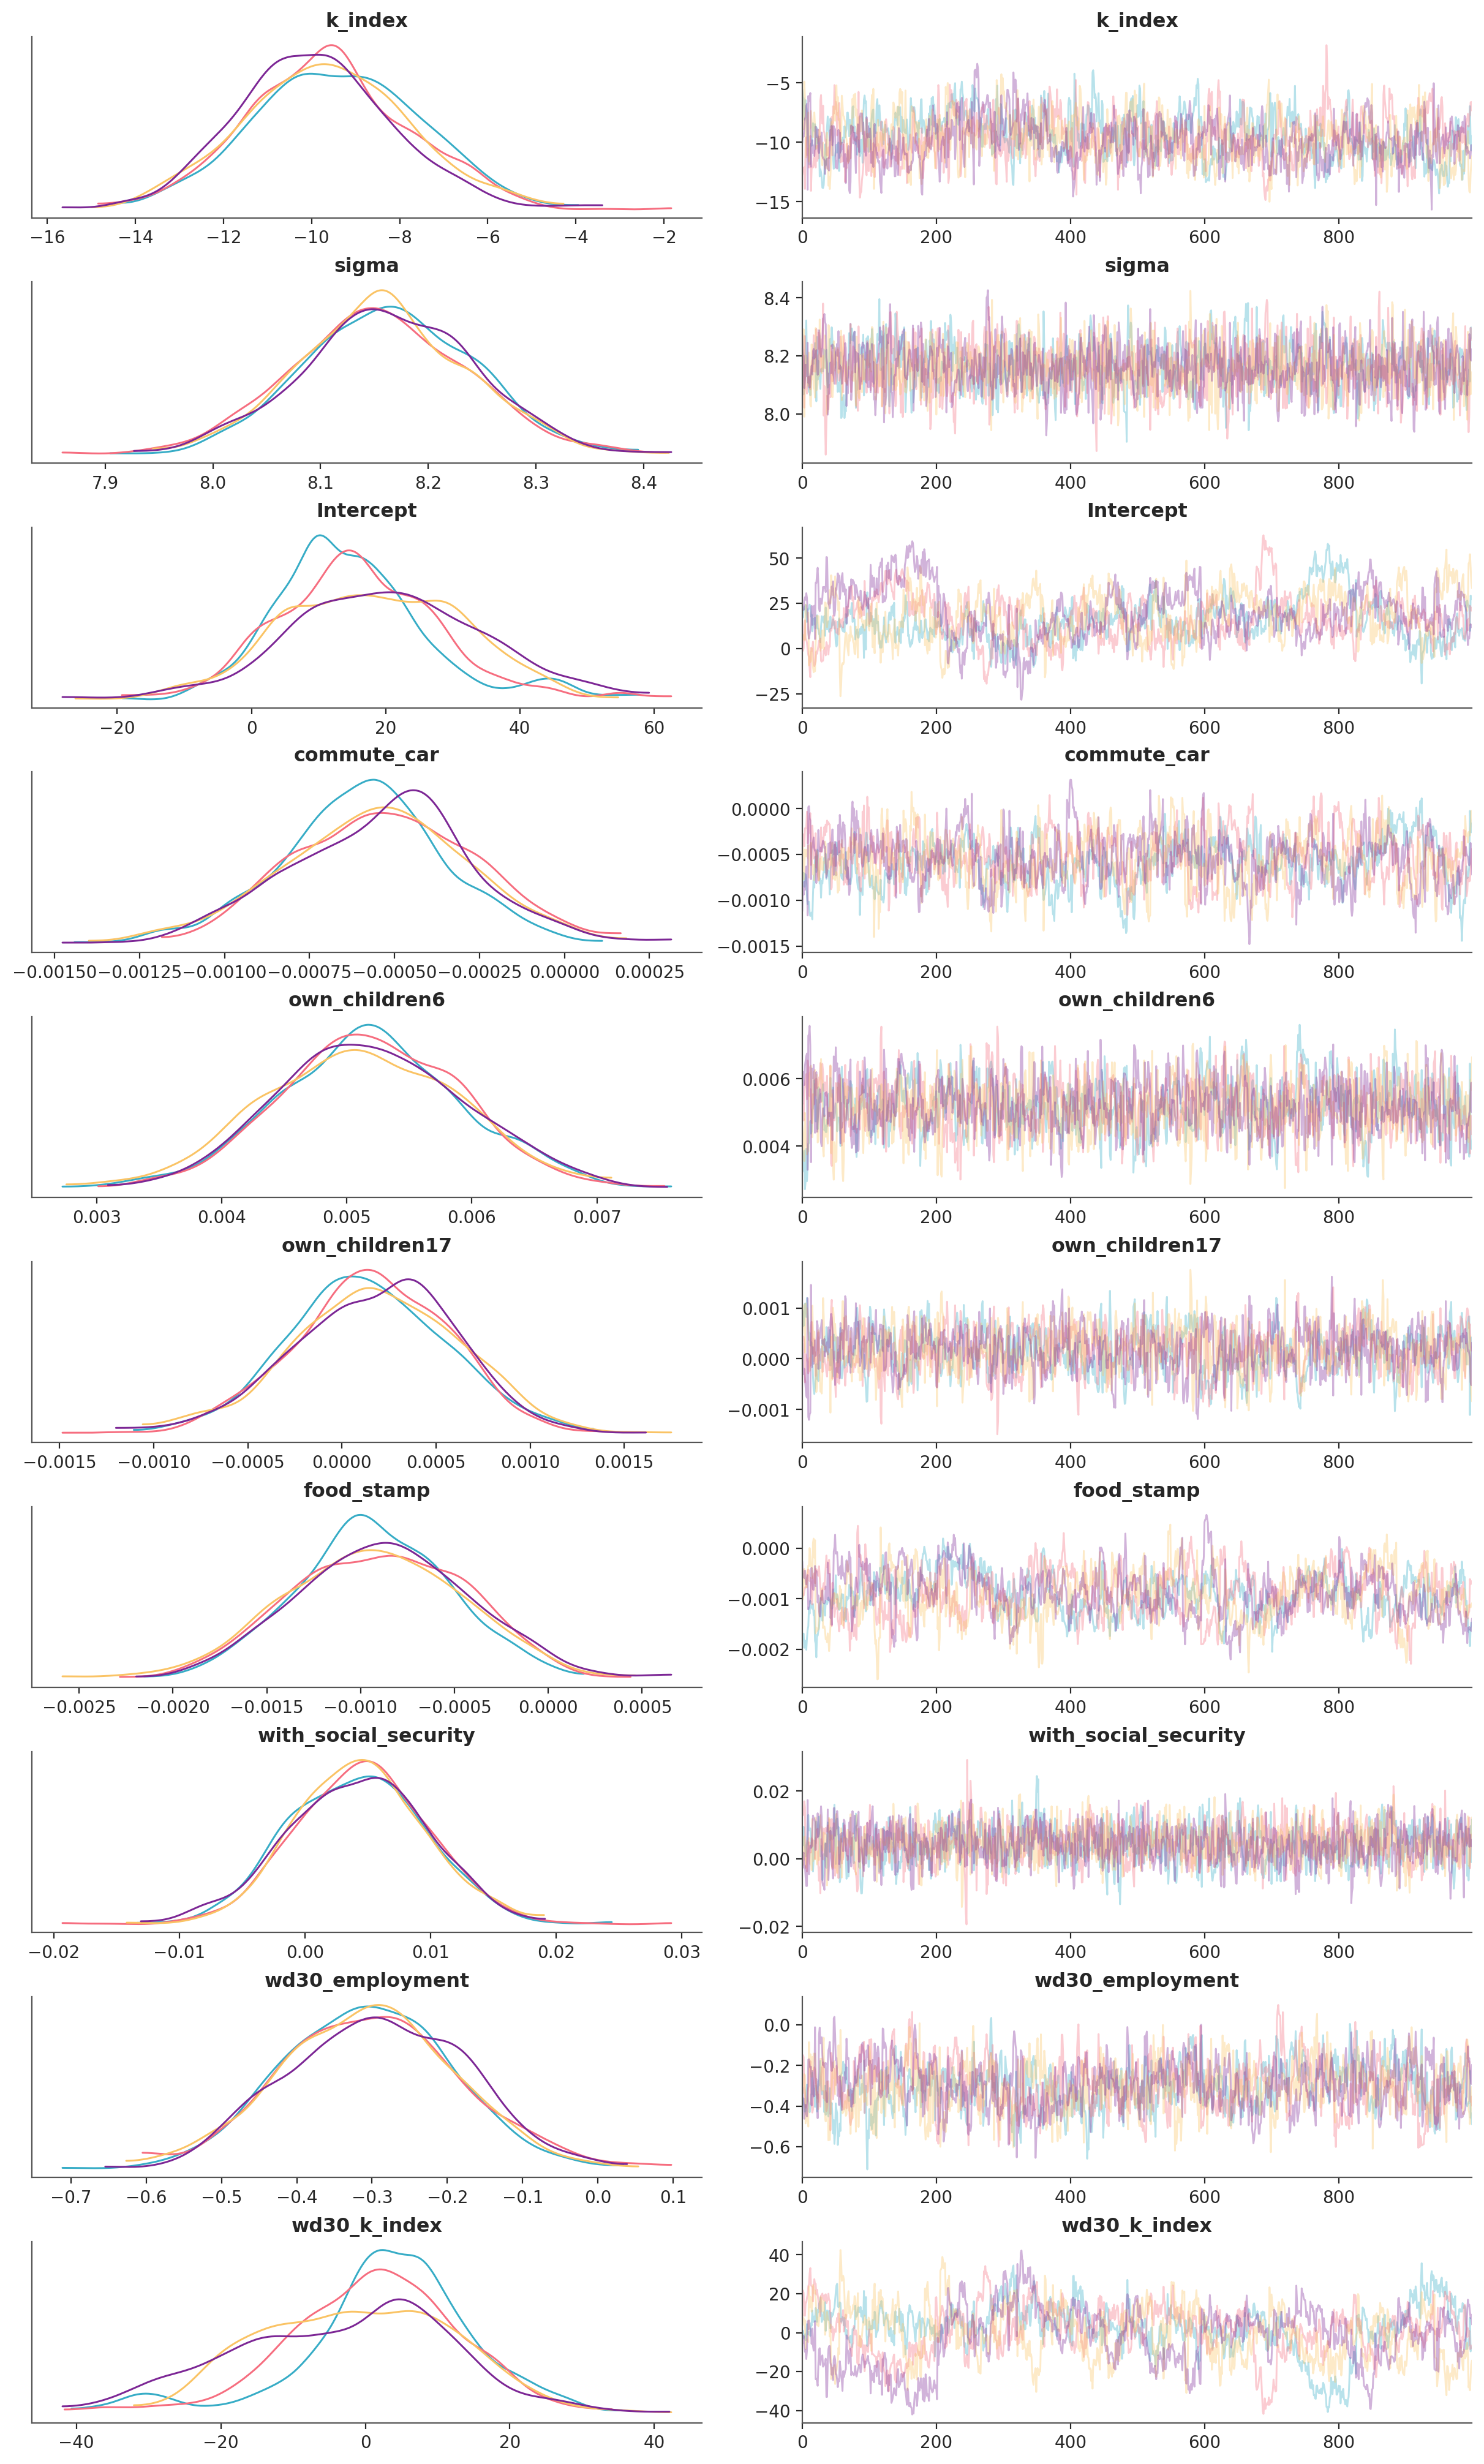
\includegraphics[width=0.4\textwidth]{assets/distance_posterior.png}
		\caption{Regression Summary (Distance)}
	\end{figure}
\end{frame}

\section{Diagnostics}
\begin{frame}{Tensor Diagnostic Plot}
	\begin{figure}
		\centering
		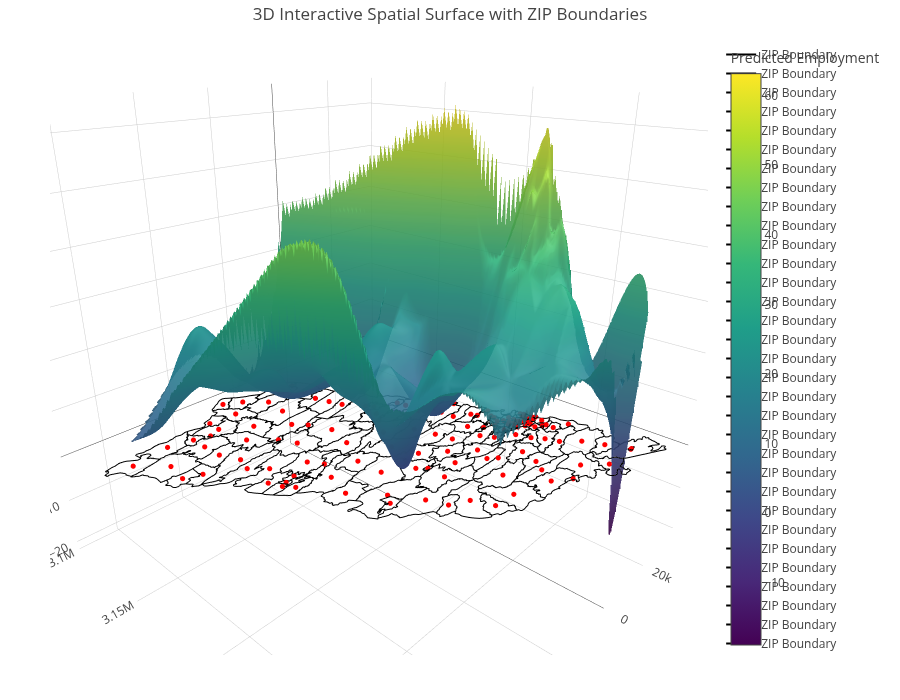
\includegraphics[width=0.4\textwidth]{assets/tensor_plot.png}
		\caption{Tensor Product Spatial Smoothing Diagnostic}
	\end{figure}
	\begin{itemize}
		\item Used to determine if spatial correlation is uniform.
		\item Results suggest non-uniform spatial relationships across centroids.
	\end{itemize}
\end{frame}

%------------------------------------------------
\section{Conclusion}
%------------------------------------------------

\begin{frame}{Key Findings \& Future Work}
	\begin{itemize}
		\item \textbf{Employment Impact:} Confirmed negative and significant relationship between Kaitz Index and employment in PR.
		\item \textbf{Spillovers:} Evidence of negative spillover effects on neighboring ZIP codes, though MCMC convergence makes magnitude precise estimation difficult.
		\item \textbf{Future Research:}
		      \begin{itemize}
			      \item Explore \textbf{lagged spatial effects}.
			      \item Utilize more complex spatial smoothing given the non-uniform nature of regional relationships.
		      \end{itemize}
	\end{itemize}
\end{frame}

\section{References}
\begin{frame}[allowframebreaks]{References}
	\printbibliography
\end{frame}

\begin{frame}
	\centering
	\Huge Thank You!
\end{frame}

\end{document}
